\section{A fixed reference box and the lower mass bound}
\label{sec:assembly}

Fix $L$ and then $H$ large enough for all preceding estimates and
for $\varepsilon_H\le1/9$ in Lemma~\ref{lem:alignment}. This choice
precedes the selection of $K_0,M_0$ and is used for both mass bounds.
All estimates needed to compare different cutoffs have now been
established. We first make that comparison at the level of actual
partition functions, then choose the reference box only once.

Let $I_H$ be the terminal interval in Proposition~\ref{rg:admission}.
For an admitted $r$-step trajectory ending at $h\in I_H$, write its
initial coupling as $\beta_r(h)$. The exact integrations and the bulk
scalar convention give
\begin{equation}
\label{eq:blocked-partition}
 Z_{\beta_r(h)}(ML^r,ML^r)
   =e^{v_r(h)M^2}\mathcal Z_{r,h}(M),\qquad
 \mathcal Z_{r,h}(M)=\int f_{r,h,M}(V)\,\dd\nu_M(V).
\end{equation}
Here $\nu_M$ is product probability measure on the coarse $M\times M$
torus, $f_{r,h,M}$ is the complete positive density, and $v_r(h)$ is
independent of $M$. Only this last independence matters; the scalar
need not converge or be close for different depths.
The notation $\beta_r(h)$ does not assert uniqueness: every estimate
is uniform over all admitted trajectories with the specified endpoints.

\begin{proposition}[Comparison of cutoffs]
\label{prop:cutoff}
There are constants $C_H,c_H,d_H>0$ and a finite depth threshold such
that, for all admitted $N\ge K$, $h\in I_H$, and dyadic
$M\ge M_{\min}(L,H)$ with $(2M)^2\le e^{c_HK}$,
\begin{equation}
\label{eq:cutoff-comparison}
 |D_N(h;M)-D_K(h;M)|\le C_He^{-d_HK},\qquad
 D_r(h;M)=\Delta_{\beta_r(h)}(ML^r).
\end{equation}
The constants do not depend on the ratio of the two bare couplings or
on $N-K$.
\end{proposition}

\begin{proof}
Theorem~\ref{rg:matching} gives a local discrepancy
$\delta_K\le C_He^{-\gamma_HK}$ for the two terminal representations.
Apply Theorem~\ref{thm:relative-comparison} with their common terminal
coupling. There is one set $G$ such that, under each normalized law,
\[
 \mu_i(G^c)\le C_HM^2e^{-a_HK},
\]
and on $G$ the logarithms of the complete densities differ by at most
\[
 C_HM^2\delta_K e^{\zeta_HK},\qquad 0<\zeta_H<\gamma_H/2.
\]
This includes the regular exponent and the signed covering sum.
Choose $c_H<\min(a_H,\gamma_H-\zeta_H)$, and decrease it if any
admissible-volume restriction requires this. Both bounds then decrease
exponentially with $K$ whenever $M^2\le e^{c_HK}$.

Lemma~\ref{cmp:normalization}, which uses the exceptional probability
under both laws, consequently gives
\[
 |\log\mathcal Z_{N,h}(M)-\log\mathcal Z_{K,h}(M)|
                  \le C_He^{-d_HK}
\]
for some $d_H>0$ and all sufficiently large $K$.
The scalar in \eqref{eq:blocked-partition} cancels exactly:
\[
 D_r(h;M)=4\log\mathcal Z_{r,h}(M)-\log\mathcal Z_{r,h}(2M),
\]
because $4M^2-(2M)^2=0$. Apply the normalization bound at $M$ and $2M$;
the factor of five is absorbed in $C_H$.
\end{proof}

The size requirement is explicit in terms of the constants in the
construction. For a prescribed coarse box and error $\varepsilon$, it
suffices that
\begin{equation}
\label{eq:K-threshold}
 K\ge\max\left\{K_{\rm adm}(L,H),\frac{2\log(2M)}{c_H},
                        \frac{\log(C_H/\varepsilon)}{d_H}\right\},
 \qquad N\ge K.
\end{equation}
Here $K_{\rm adm}$ includes both trajectory admission and the lower
depth threshold in Proposition~\ref{prop:cutoff}.
Calibration gives
\begin{equation}
\label{eq:beta-depth}
 \beta_r(h)=\frac{\log L}{\pi}r+\frac1{2\pi}\log r+O_{L,H}(1).
\end{equation}
Thus the shorter depth controls the required largeness of both bare
inverse couplings. The proof gives finite thresholds through a specified
order of inequalities; it does not supply a useful numerical value for
them. The two trajectories must have the same terminal kinetic
coupling. Mere largeness of two arbitrarily chosen bare couplings is
not that matching condition.

\begin{theorem}[Lower bound]
\label{thm:lower}
There are fixed $K_0,M_0$, independent of the final depth, such that
\begin{equation}
\label{eq:lower-depth}
 \gap(\beta_N(h))\ge\frac{\log2}{M_0L^N},
 \qquad N\ge K_0,\quad h\in I_H.
\end{equation}
In particular $\gap(\beta)\ge c\sqrt\beta e^{-\pi\beta}$ for every
sufficiently large bare coupling, with $c>0$.
\end{theorem}

\begin{proof}
Temporarily let the reference depth $K$ grow. Choose a dyadic $M_K$ with
$\log M_K=K^{3/4}+O(1)$, and put $n_K=M_KL^K$.
Since $\log M_K=o(K)$, Proposition~\ref{prop:cutoff} admits $M_K$ and
$2M_K$ for all large $K$. By calibration and
Theorem~\ref{thm:preliminary}, uniformly for $h\in I_H$,
\[
 \log\frac{n_K}{\Xi(\beta_K(h))}
 =K^{3/4}-O_{L,H}(\sqrt{K\log K})\longrightarrow+\infty.
\]
The ratio grows faster than every polynomial in $K$, whereas the
logarithm of the polynomial prefactor in the preliminary estimate is
only $O_{L,H}(K)$. Hence
\[
 \sup_{h\in I_H}D_K(h;M_K)\longrightarrow0.
\]
Choose one finite $K_0$ for which all admissibility requirements hold
and
\[
 \sup_{h\in I_H}D_{K_0}(h;M_{K_0})+C_He^{-d_HK_0}\le2^{-10}.
\]
Fix $M_0=M_{K_0}$. The cutoff comparison now gives
$D_N(h;M_0)\le2^{-10}$ for every $N\ge K_0$.
Proposition~\ref{prop:criterion}, and uniqueness of the periodic limit
from Theorem~\ref{thm:preliminary}, prove \eqref{eq:lower-depth}.
Neither the reference depth nor the coarse box subsequently changes.

Finally, \eqref{eq:calibration} identifies $L^{-N}$ with
$\sqrt\beta e^{-\pi\beta}$ up to fixed positive factors.
Proposition~\ref{rg:admission} covers every sufficiently large bare
coupling, so this proves the last assertion.
\end{proof}

Figure~\ref{fig:fixed-reference-box} summarizes the order of choices.
\begin{figure}[tbp]
  \centering
  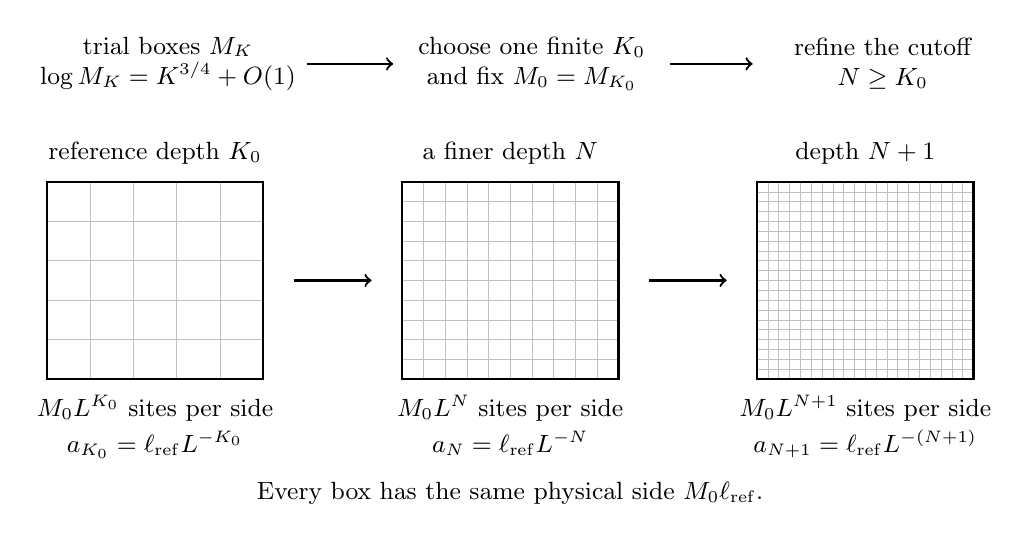
\begin{tikzpicture}[x=1.1cm,y=1cm,font=\small]
    \node[align=center] at (1.4,4.0)
      {trial boxes $M_K$\\$\log M_K=K^{3/4}+O(1)$};
    \draw[->,thick] (3.0,4.0) -- (4.0,4.0);
    \node[align=center] at (5.6,4.0)
      {choose one finite $K_0$\\and fix $M_0=M_{K_0}$};
    \draw[->,thick] (7.2,4.0) -- (8.15,4.0);
    \node[align=center] at (9.65,4.0)
      {refine the cutoff\\$N\ge K_0$};

    \begin{scope}[shift={(0,0)}]
      \draw[step=0.5,black!25,very thin] (0,0) grid (2.5,2.5);
      \draw[thick] (0,0) rectangle (2.5,2.5);
      \node[above] at (1.25,2.6) {reference depth $K_0$};
      \node[align=center,below] at (1.25,-0.08)
        {$M_0L^{K_0}$ sites per side\\[2pt]$a_{K_0}=\ell_{\mathrm{ref}}L^{-K_0}$};
    \end{scope}
    \draw[->,thick] (2.85,1.25) -- (3.75,1.25);
    \begin{scope}[shift={(4.1,0)}]
      \draw[step=0.25,black!25,very thin] (0,0) grid (2.5,2.5);
      \draw[thick] (0,0) rectangle (2.5,2.5);
      \node[above] at (1.25,2.6) {a finer depth $N$};
      \node[align=center,below] at (1.25,-0.08)
        {$M_0L^N$ sites per side\\[2pt]$a_N=\ell_{\mathrm{ref}}L^{-N}$};
    \end{scope}
    \draw[->,thick] (6.95,1.25) -- (7.85,1.25);
    \begin{scope}[shift={(8.2,0)}]
      \draw[step=0.125,black!25,very thin] (0,0) grid (2.5,2.5);
      \draw[thick] (0,0) rectangle (2.5,2.5);
      \node[above] at (1.25,2.6) {depth $N+1$};
      \node[align=center,below] at (1.25,-0.08)
        {$M_0L^{N+1}$ sites per side\\[2pt]$a_{N+1}=\ell_{\mathrm{ref}}L^{-(N+1)}$};
    \end{scope}
    \node at (5.35,-1.45)
      {Every box has the same physical side $M_0\ell_{\mathrm{ref}}$.};
  \end{tikzpicture}\par\medskip
  \caption{The order of choices in the lower-bound argument.
  The growing family of trial boxes is used only to select one
  reference depth and one coarse period. The comparison then transfers
  the small square-box test to all finer admitted cutoffs at the same
  terminal coupling. The grids are schematic; their counts are not
  the actual lattice periods. Refinement does not enlarge the physical
  reference box.}
  \label{fig:fixed-reference-box}
\end{figure}


The exponent $3/4$ is only a convenient choice between $1/2$ and $1$.
More generally an error $o(\beta)$ in the logarithm of the preliminary
length can be absorbed in a subexponentially growing reference box.
Calibration fixes the physical size of a coarse cell; comparison
transfers a small partition-function test to a fixed number of those
cells. Both facts are needed for the bound.

